\section{Introduction to kinematics}
Objectives:
\begin{enumerate}
  \item Course overview
  \item Key terminology
    \item Graphing motion
\end{enumerate}

\subsection{Overview}
We'll start the semester by learning about kinematics. Kinematics is the description of motion, and has the same origins as the word cinema. In a few weeks we'll discuss dynamics, or causes of motion. When we combine kinematics with dynamics, we are studying mechanics. In introductory physics, we'll cover classical mechanics --- one of the oldest branches of science

Classical mechanics: large, slow moving objects\\
Quantum mechanics: small objects\\
General relativity: fast moving objects\\

[Insert diagram of physics disciplines.]
\vspace{5cm}

\subsection{Types of motion}
motion: change in object's position with time

trajectory: path along which an object travels

For now, we'll only worry about rigid body motion (i.e., no deformation).

Four special cases of motion:

\begin{itemize}
\item straight line
\item projectile motion (influenced by gravity)
\item circular motion (e.g., planets, satellites)
\item rotational motion
\end{itemize}

\clearpage
[Insert diagrams.]
\vspace{6cm}

For motion that does not involve deformation or rotation, we can use a \textit{particle model}. Models are simplifications of reality that allow us to focus on important physics. In a particle model, we assume that all of the mass of an object is focused at a single point and that the all parts of the object move in the same direction with the same speed. Particle models are a good approximation of rigid body motion. In class I'll often use particles and boxes to represent much more complicated objects.

\subsection{Terms used to describe motion}
\begin{itemize}
\item position = location of an object

[Insert 1-D diagram; where is the object on this line?]
\vspace{3cm}


position can be positive \textit{or} negative -- this is important\\
units = [L]

\item displacement = change in position, [L] 
$$\Delta{x}=x_f-x_i$$
Can be positive \textit{or} negative (give example).

\item average velocity = average rate of change of position, [L]/[T]
$$v=\frac{\Delta{x}}{\Delta{t}}=\frac{x_f-x_i}{t_f-t_i}$$
Velocity can ALSO be positive \textit{or} negative. What does the sign tell you?

\item average speed = magnitude of average velocity, [L]/[T], always positive

\clearpage
Example: plot of position vs. time

[Insert diagram.]
\vspace{4cm}

Average velocity during the first interval:
$$v_1=\frac{x_1-x_0}{t_1-t_0}\Rightarrow\mbox{ slope of a straight line}$$
$$v_1>0$$

Average velocity during the second interval:
$$v_2=\frac{x_2-x_1}{t_2-t_1}<0$$

Often, we are more interested in the instantaneous velocity -- which means that calculus will already come in handy! Anybody know how?
$$\boxed{v=\lim_{\Delta{t}\rightarrow{0}}\frac{\Delta{x}}{\Delta{t}}=\frac{dx}{dt}}\Rightarrow\mbox{ evaluate at some point in time}$$

In practice, data is not continuous, velocity calculated from data is an average over some time interval.

From the fundamental theorem of calculus, we can see how displacement is related to velocity. (We won't do a lot of work with integrals, this is mostly for completeness.)
$$v=\frac{dx}{dt}\Rightarrow \boxed{\int_{t_0}^{t_1}v\,dt = \int_{t_0}^{t_1}\frac{dx}{dt}\,dt=x(t_1)-x(t_0)=\Delta{x}}$$


\item average acceleration = average rate of change of velocity, [L]/[T$^2$]
$$a_{avg}=\frac{v_2-v_1}{t_2-t_1}=\frac{\Delta{v}}{\Delta{t}}$$
As with velocity, often we are interested in the instantaneous acceleration
$$a=\lim_{\Delta{t}\rightarrow 0}\frac{\Delta{v}}{\Delta{t}}=\frac{dv}{dt}$$
Sometimes written as a second derivative
$$a=\frac{dv}{dt}=\frac{d\frac{dx}{dt}}{dt}=\frac{d^2x}{dt^2}$$
Not surprisingly, given what we just saw with displacement,
$$\Delta{v}=\int_{t_0}^{t_1}a\,dt$$
Can also be positive \textit{or} negative. What does the sign mean?

Simple rule for determining whether an object is accelerating or decelerating:\\
If $a\cdot v>0$ the object is accelerating, if $a\cdot v<0$ the object is decelerating  
\end{itemize}

\subsection{Example problems}

\begin{itemize}
\item The position of a particle, in cm, is given by $x(t)=9.75+1.50t^3$. (i) Sketch the position, velocity, and acceleration curves. (ii) What is the velocity at $t=2$s? What is the acceleration at $t=2$s? 

  \vspace{5cm}

\item A ball rolls along a smooth track shown in the figure. Each segment of the track is straight, and the ball passes smoothly from one segment to the next without changing speed or leaving the track. Draw three vertically stacked graphs showing position, velocity, and acceleration versus time. Each graph should have the same time axis, the proportions of the graph should be qualitatively correct. Assume that the ball has enough speed to reach the top.

  \begin{figure}[h]
    \begin{center}
      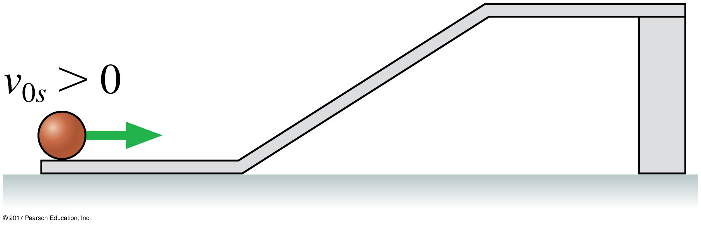
\includegraphics[]{./figs/P02_43_Figure.pdf}
    \end{center}  
  \end{figure}
  
  \end{itemize}

\clearpage
